
\begin{figure}
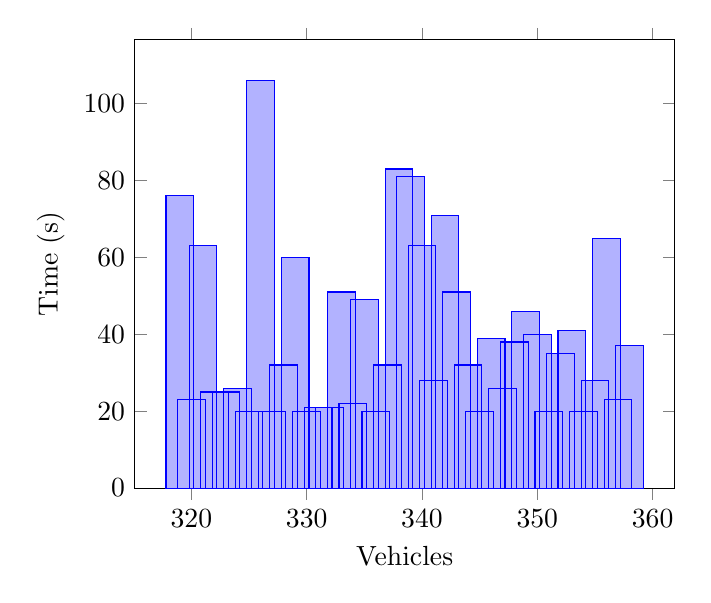
\begin{tikzpicture}
\begin{axis}[
legend style={anchor=west},
xlabel=Vehicles,
ylabel=Time (s),
ymin=0,
ybar,
]
\addplot coordinates {
(334, 22)
(342, 71)
(341, 28)
(349, 46)
(352, 35)
(353, 41)
(324, 26)
(339, 81)
(337, 32)
(330, 20)
(340, 63)
(338, 83)
(346, 39)
(320, 23)
(326, 106)
(325, 20)
(332, 21)
(335, 49)
(356, 65)
(357, 23)
(351, 20)
(344, 32)
(323, 25)
(355, 28)
(322, 25)
(347, 26)
(354, 20)
(345, 20)
(327, 20)
(329, 60)
(331, 21)
(348, 38)
(343, 51)
(336, 20)
(358, 37)
(350, 40)
(321, 63)
(333, 51)
(328, 32)
(319, 76)
};

\end{axis}
\end{tikzpicture}
\label{tik:time:100:78}
\caption{100 percent diving with GSC on route $78$}
\end{figure}
